\section{Latches}

All logic circuits discussed so far have been directed acyclic graphs: data flow
in a single direction for each connection and any individual signal starts at
one of the inputs and travels through the graph to one of the outputs, never
passing through the same gate more than once.  This is enough to implement
transient computation, such as additions and bitwise operations, as we have
seen, but computers also need to \emph{retain} information for a period of time.
Building components which can do that requires some form of loop where the
current state is used in the computation of the next.

A very simple circuit with that property is an \textit{or} gate whose output is
connected to one of its inputs (figure \ref{fig:arch:or_loop}).  The output of
this circuit will be zero until the input is set.  From that point on, as long
as the circuit is powered, its output will always be on, since the signal that
loops back to the \textit{or} gate is on and that is enough to turn the gate on.

\begin{figure}[p]
    \centering
    \begin{subfigure}{0.24\textwidth}
        \input{arch/latches/or_loop0.tex}
        \caption{initial state}
    \end{subfigure}
    \begin{subfigure}{0.24\textwidth}
        \input{arch/latches/or_loop1.tex}
        \caption{input is set}
    \end{subfigure}
    \begin{subfigure}{0.24\textwidth}
        \begin{tikzpicture}[{circuit_diagram}]
    \node (or) [or gate] {};
    \node (in) [left = of or.input 1, xshift = 1em] {I};
    \node (or0) [point, right = of or, xshift = -2em] {};
    \node (out) [right = of or0, xshift = -2em] {O};
    \draw [red, thick] (in) -- (or.input 1);
    \draw [red, thick] (or.output) -- (or0);
    \draw [red, thick] (or0) -- (out);
    \draw [red, thick] (or0)
        -- ($
            (0, -0.6)
            + (0, 0)!(or0)!(1, 0)
            + (0, 0)!(or.input 2)!(0, 1)
        $)
        -- ($ (or.input 2) - (0.4, 0.6) $)
        -- ($ (or.input 2) - (0.4, 0) $)
        -- (or.input 2);
\end{tikzpicture}

        \caption{\textit{or} propagates}
    \end{subfigure}
    \begin{subfigure}{0.24\textwidth}
        \input{arch/latches/or_loop3.tex}
        \caption{input is cleared}
    \end{subfigure}
    \caption{\textit{or} gate with a loop}
    \label{fig:arch:or_loop}
\end{figure}

Figure \ref{fig:arch:sr_latch} shows an improved version of this concept where
two \textit{nor} gates are interconnected.  Initially, one of the two outputs,
which are complements, is set (which one depends on propagation delays, this is
a hardware race condition).

\begin{figure}[p]
    \centering
    \begin{subfigure}{0.25\textwidth}
        \begin{tikzpicture}[scale = 0.75, circuit logic CDH, huge circuit symbols]
    \node (q)  at (0, 2) {Q};
    \node (nq) at (0, 0) {$\bar{\text{Q}}$};
    \node (nor0) [nor gate, left = of q] {};
    \node (nor1) [nor gate, left = of nq] {};
    \node (p0) [point, right = of nor0.output, xshift = -1.75em] {};
    \node (p1) [point, right = of nor1.output, xshift = -1.75em] {};
    \node (r) [left = of nor0.input 1, xshift = 1em] {R};
    \node (s) [left = of nor1.input 2, xshift = 1em] {S};
    \draw (r) -- (nor0.input 1);
    \draw (s) -- (nor1.input 2);
    \draw [red, thick] (p0)
        -- ($ (nor1.input 1) + (-1em, 1em) $)
        -- ($ (nor1.input 1) - (1em, 0) $)
        -- (nor1.input 1);
    \draw (p1)
        -- ($ (nor0.input 2) - (1em, 1em) $)
        -- ($ (nor0.input 2) - (1em, 0) $)
        -- (nor0.input 2);
    \draw [red, thick] (nor0.output) -- (q);
    \draw (nor1.output) -- (nq);
\end{tikzpicture}

        \caption{initial state}
    \end{subfigure}
    \begin{subfigure}{0.25\textwidth}
        \input{arch/latches/flip_flop1.tex}
        \caption{reset is raised}
    \end{subfigure}
    \begin{subfigure}{0.25\textwidth}
        \input{arch/latches/flip_flop2.tex}
        \caption{Q is cleared}
    \end{subfigure}
    \\~\\~\\
    \begin{subfigure}{0.25\textwidth}
        \input{arch/latches/flip_flop3.tex}
        \caption{$\bar{\text{Q}}$ is set}
    \end{subfigure}
    \begin{subfigure}{0.25\textwidth}
        \input{arch/latches/flip_flop4.tex}
        \caption{reset is lowered}
    \end{subfigure}
    \begin{subfigure}{0.25\textwidth}
        \input{arch/latches/flip_flop5.tex}
        \caption{set is raised}
    \end{subfigure}
    \\~\\~\\
    \begin{subfigure}{0.25\textwidth}
        \input{arch/latches/flip_flop6.tex}
        \caption{$\bar{\text{Q}}$ is cleared}
    \end{subfigure}
    \begin{subfigure}{0.25\textwidth}
        \input{arch/latches/flip_flop7.tex}
        \caption{Q is set}
    \end{subfigure}
    \begin{subfigure}{0.25\textwidth}
        \input{arch/latches/flip_flop8.tex}
        \caption{set is lowered}
    \end{subfigure}
    \caption{SR latch}
    \label{fig:arch:sr_latch}
\end{figure}

Assuming that is the gate associated with R, the circuit will reach a stable
state where Q is set.  Raising and lowering S at this point has no effect, as
the \textit{nor} gate will not propagate the signal as long as the crossed
connection is on.  Raising R (short for \textit{reset}) will clear Q, but also
clear the input to the other \textit{nor} gate.  This will cause both
$\bar{\text{Q}}$ and one of the inputs to the first \textit{nor} gate to be set.
R can be lowered and raising and lowering it again at this point has no effect.
Raising S (short for \textit{set}) has the opposite effect: $\bar{\text{Q}}$ and
the first gate are cleared, Q is set, and we are back at the initial state.

From this we can observe that the circuit has two stable states: Q set and
$\bar{\text{Q}}$ cleared, or vice versa.  Raising R or S transitions the circuit
from one state to the other, which will be maintained until the next transition.
Components that exhibit this type of behavior are called \textit{latches}, as
the output is locked when an operation is performed and state is preserved.
This particular circuit is called an \textit{SR latch}, due to its two inputs.

The \textit{D latch} (figure \ref{fig:arch:d_latch}) is a similar circuit which
uses a single input instead of a reset/set pair.  Two additions to the SR latch
accomplish this.  First, a single input D (short for \textit{data}) is connected
to R and S, with R going through a \textit{not} gate.  State is now no longer
retained since toggling D immediately raises one of R or S.  An input EN (short
for \textit{enable}) is added so that transitions occur only when it is on.
This is done by placing two \textit{and} gates between R/S and the latch, which
are also connected to EN.

\begin{figure}[p]
    \centering
    \begin{tikzpicture}[circuit logic CDH, huge circuit symbols]
    \node (q)  at (6, 2) {Q};\node (nq) at (6, 0) {$\bar{\text{Q}}$};
    \node (nor0) [nor gate, left = of q] {};
    \node (nor1) [nor gate, left = of nq] {};
    \node (and0) [and gate, left = of nor0.input 1, xshift = 1em] {R};
    \node (and1) [and gate, left = of nor1.input 2, xshift = 1em] {S};
    \node (p0) [point, right = of nor0.output, xshift = -1.75em] {};
    \node (p1) [point, right = of nor1.output, xshift = -1.75em] {};
    \node (not) [
        not gate, circuit symbol unit = 0.4em,
        left = of and0.input 1, xshift = 1em,
    ] {};
    \node (d0) [point] at (0, 1) {};
    \node (d) [left = of d0, xshift = 2em] {D};
    \node (en0) [point] at (1.25, 1) {};
    \node (en) [left = of en0, xshift = 2em] {EN};
    \draw (d) -- (d0);
    \draw (d0) |- (not) -- (and0.input 1);
    \draw (d0) |- (and1.input 2);
    \draw (en) -- (en0);
    \draw (en0) |- (and0.input 2);
    \draw (en0) |- (and1.input 1);
    \draw (and0) -- (nor0.input 1);
    \draw (and1) -- (nor1.input 2);
    \draw (p0)
        -- ($ (nor1.input 1) + (-1em, 1em) $)
        -- ($ (nor1.input 1) - (1em, 0) $)
        -- (nor1.input 1);
    \draw (p1)
        -- ($ (nor0.input 2) - (1em, 1em) $)
        -- ($ (nor0.input 2) - (1em, 0) $)
        -- (nor0.input 2);
    \draw (nor0.output) -- (q);
    \draw (nor1.output) -- (nq);
    \draw[-, dotted]
        ($ (and1)    + (-0.75em, -1.50em) $)
        -- node[below] {latch} +(12.25em, 0)
        -- ($ (and0) + (11.50em,  1.50em) $)
        -- ($ (and0) + (-0.75em,  1.50em) $)
        -- ($ (and1) + (-0.75em, -1.50em) $);
\end{tikzpicture}

    \caption{D latch}
    \label{fig:arch:d_latch}
\end{figure}

These additions create a circuit that will change its state based on the
combination of both its inputs.  Figure \ref{fig:arch:d_latch_clock} shows the
relationship between changes to D/EN and the output of a D latch over time.
Whenever EN is on, Q follows the value of D (green lines).  Conversely, changing
D while EN is off has no effect on the value of Q (red lines).  This type of
latch is called a \textit{transparent latch}, as the value of the input is
constantly forwarded to the output as long as the enable signal is on.

\begin{figure}[ht]
    \centering
    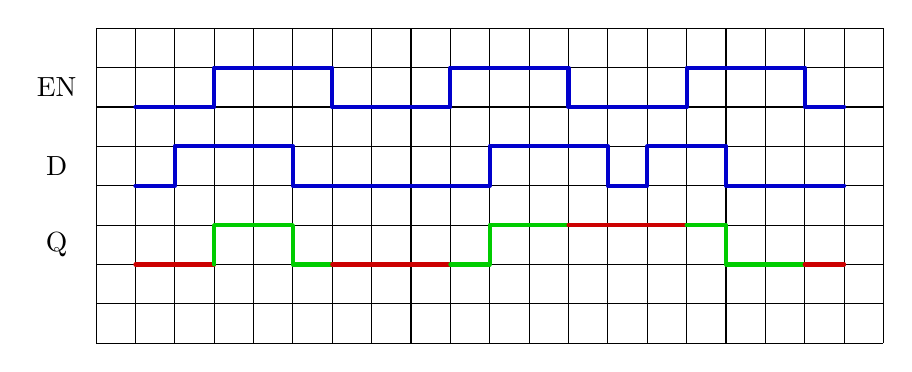
\begin{tikzpicture}[
        scale = 0.5,
        line/.style={line width = 0.15em, line join = round, line cap = round},
        input/.style={line, blue!80!black},
        on/.style={line, green!80!black},
        off/.style={line, red!80!black},
    ]
        \draw[step = 1] (0, 0) grid (20, 8);
        \node at (-1, 6.5) {EN};
        \node at (-1, 4.5) {D};
        \node at (-1, 2.5) {Q};
        \draw[input]
            (1, 6) -- (3, 6) -- (3, 7) -- (6, 7) -- (6, 6) -- (9, 6) -- (9, 6)
            -- (9, 7) -- (12, 7) -- (12, 6) -- (15, 6) -- (15, 7) -- (18, 7)
            -- (18, 6) -- (19, 6);
        \draw[input]
            (1, 4) -- (2, 4) -- (2, 5) -- (5, 5) -- (5, 4) -- (10, 4) -- (10, 5)
            -- (13, 5) -- (13, 4) -- (14, 4) -- (14, 5) -- (16, 5) -- (16, 4)
            -- (19, 4);
        \draw[off] ( 1, 2) -- ( 3, 2);
        \draw[on]  ( 3, 2) -- ( 3, 3) -- ( 5, 3) -- ( 5, 2) -- (6, 2);
        \draw[off] ( 6, 2) -- ( 9, 2);
        \draw[on]  ( 9, 2) -- (10, 2) -- (10, 3) -- (12, 3);
        \draw[off] (12, 3) -- (15, 3);
        \draw[on]  (15, 3) -- (16, 3) -- (16, 2) -- (18, 2);
        \draw[off] (18, 2) -- (19, 2);
    \end{tikzpicture}
    \caption{D latch timing diagram}
    \label{fig:arch:d_latch_clock}
\end{figure}

\begin{figure}[ht]
    \centering
    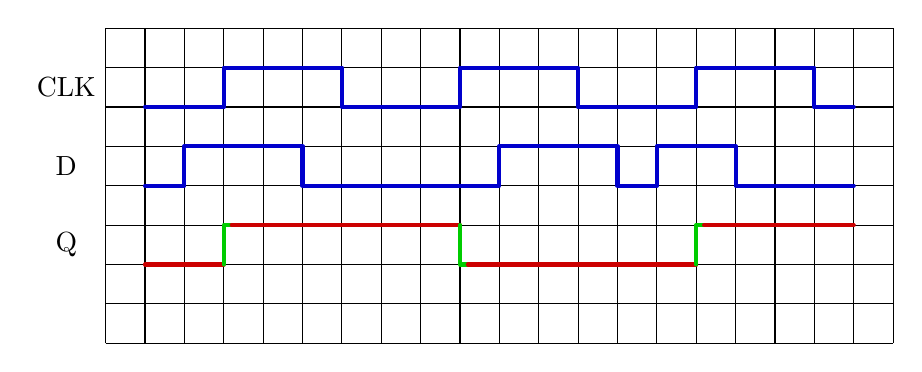
\begin{tikzpicture}[
        scale = 0.5,
        line/.style={line width = 0.15em, line join = round, line cap = round},
        input/.style={line, blue!80!black},
        on/.style={line, green!80!black},
        off/.style={line, red!80!black},
    ]
        \draw[step = 1] (0, 0) grid (20, 8);
        \node at (-1, 6.5) {CLK};
        \node at (-1, 4.5) {D};
        \node at (-1, 2.5) {Q};
        \draw[input]
            (1, 6) -- (3, 6) -- (3, 7) -- (6, 7) -- (6, 6) -- (9, 6) -- (9, 6)
            -- (9, 7) -- (12, 7) -- (12, 6) -- (15, 6) -- (15, 7) -- (18, 7)
            -- (18, 6) -- (19, 6);
        \draw[input]
            (1, 4) -- (2, 4) -- (2, 5) -- (5, 5) -- (5, 4) -- (10, 4) -- (10, 5)
            -- (13, 5) -- (13, 4) -- (14, 4) -- (14, 5) -- (16, 5) -- (16, 4)
            -- (19, 4);
        \draw[off] ( 1.0, 2) -- ( 3, 2);
        \draw[on]  ( 3.0, 2) -- ( 3, 3) -- (3.2, 3);
        \draw[off] ( 3.2, 3) -- ( 9, 3);
        \draw[on]  ( 9.0, 3) -- ( 9, 2) -- (9.2, 2);
        \draw[off] ( 9.2, 2) -- (15, 2);
        \draw[on]  (15,   2) -- (15, 3) -- (15.2, 3);
        \draw[off] (15.2, 3) -- (19, 3);
    \end{tikzpicture}
    \caption{Flip-flop timing diagram}
    \label{fig:arch:flip_flop_clock}
\end{figure}

A more common design in computers is to have components synchronize state
changes according to a regular, intermittent signal: a \textit{clock}.  In this
scenario, we want latches to update their state at the \emph{edge} of the clock
signal, i.e. right when it changes its state --- either from zero to one, the
\textit{rising edge}, or from one to zero, the \textit{falling edge}.  Figure
\ref{fig:arch:flip_flop_clock} shows a timing diagram with the same input, but
with Q transitions happening at the clock rise signal.  The intervals in which D
influences the value of Q (green lines again) are now very short and even more D
transitions are ignored.

A simple circuit that can identify the rising edge of a clock signal, an
\textit{edge detection circuit}, is shown in figure \ref{fig:arch:edge_detect}.
At first it might seem like a circuit that never outputs anything, but the small
delay introduced by the \textit{not} gate allows the output to be turned on
momentarily.  More \textit{not} gates can be added to increase the interval in
which the input signal is allowed to be propagated.  Other types of edge
detection circuits are possible, such as placing a capacitor and a resistor
between the input and output.  Substituting the EN input of a latch with such an
edge detector creates a component called a \textit{flip-flop}, which otherwise
operates in the same way: a transparent latch is \textit{level-triggered}, while
a flip-flop is \textit{edge-triggered}.  These are the basic building blocks for
storing data in a logic circuit.

\begin{figure}[ht]
    \centering
    \begin{tikzpicture}[{circuit_diagram}]
        \node (and) [and gate] {};
        \node (not) [
            not gate, circuit symbol unit = 0.4em,
            left = of and.input 2, xshift = 2em,
        ] {};
        \node (in0) [point, left = of and] {};
        \node (in)  [left = of in0, xshift = 2em] {I};
        \node (out) [right = of and, xshift = -2em] {O};
        \draw (in) -- (in0);
        \draw (in0) |- (and.input 1);
        \draw (in0) |- (not.input);
        \draw (not.output) -- (and.input 2);
        \draw (and.output) -- (out);
    \end{tikzpicture}
    \caption{\textit{and}/\textit{not} gate edge detector}
    \label{fig:arch:edge_detect}
\end{figure}
